\documentclass{beamer}

\usepackage{changepage}
\usepackage{hyperref}

\usepackage[skip=0.2\baselineskip]{parskip}

\usepackage{mathrsfs}
\usepackage{caption}
\usepackage{subcaption}
\usepackage{tikz}
\usepackage{makecell}
\usepackage{array,booktabs}
\newcolumntype{C}{>{$\displaystyle}c<{$}}

\setlength\fboxsep{0pt}
\setlength\fboxrule{0pt}



\usepackage{beamerthemepamango-blank}
\usepackage{shortcuts_pm}

\usepackage{marvosym}

\setbeamertemplate{caption}{\raggedright\insertcaption\par}

\addbibresource{references.bib}

%%%%% INFORMATION

\title{\Huge Learning Privately\\ in High Dimension}
\author{
  Paul Mangold \\[1em]
 (Aurélien~Bellet, Marc~Tommasi, Joseph~Salmon)
}
\institute{\textsc{DATING Seminar}}

\date{October 11th, 2022}

%%%%% DOCUMENT

\begin{document}

%% TITLE PAGE

\begin{notitle}
  \begin{frame}
    \titlepage
  \end{frame}
  \addtocounter{framenumber}{-1}
\end{notitle}

\begin{frame}
  \vspace{1em}
  \begin{center}
    \Huge
    Supervised Learning

    \vspace{1em}

    \begin{tikzpicture}
      \node[anchor=south west,inner sep=0] (cat1) at (0,4.5) {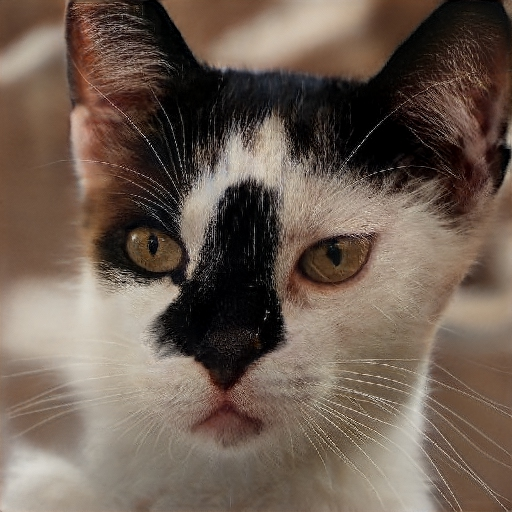
\includegraphics[width=0.1\textwidth]{dogs_cats/cat1.jpeg}};
      \node[anchor=south west,inner sep=0] (cat2) at (0,3) {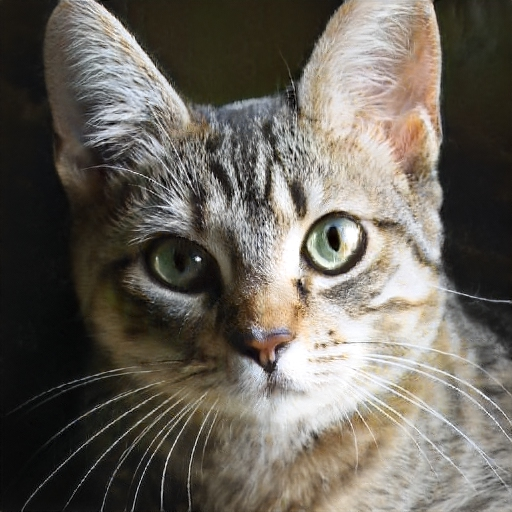
\includegraphics[width=0.1\textwidth]{dogs_cats/cat2.jpeg}};
      \node[anchor=south west,inner sep=0] (cat3) at (0,1.5) {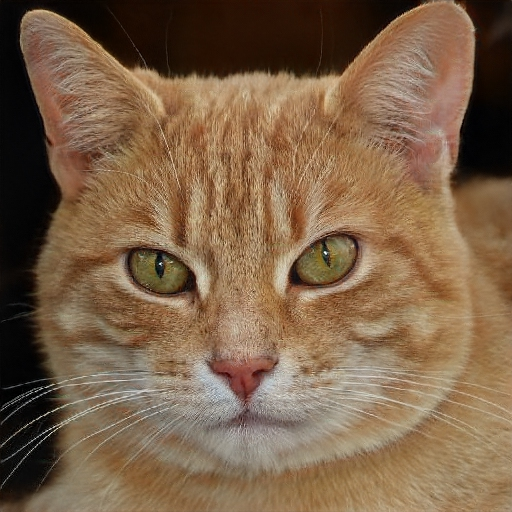
\includegraphics[width=0.1\textwidth]{dogs_cats/cat3.jpeg}};
      \node[anchor=south west,inner sep=0] (dog1) at (0,0) {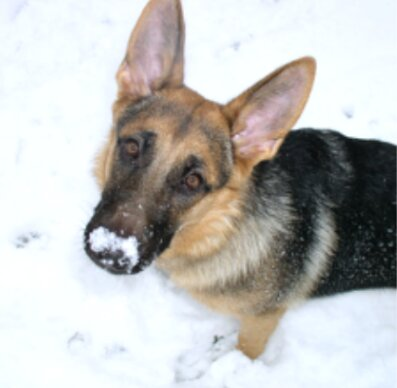
\includegraphics[width=0.1\textwidth]{dogs_cats/dog1.jpeg}};
      \only<2>{
      \node[anchor=south west,inner sep=0] (name1) at (2,4.75) {cat};
      \node[anchor=south west,inner sep=0] (name2) at (2,3.25) {cat};
      \node[anchor=south west,inner sep=0] (name3) at (2,1.75) {cat};
      \node[anchor=south west,inner sep=0] (name4) at (2,0.25) {dog};
      \draw [-latex,shorten >= 3pt, shorten <= 3pt, amaranth, ultra thick] (cat1) to (name1);
      \draw [-latex,shorten >= 3pt, shorten <= 3pt, amaranth, ultra thick] (cat2) to (name2);
      \draw [-latex,shorten >= 3pt, shorten <= 3pt, amaranth, ultra thick] (cat3) to (name3);
      \draw [-latex,shorten >= 3pt, shorten <= 3pt, amaranth, ultra thick] (dog1) to (name4);}
  \end{tikzpicture}%

  \end{center}

\end{frame}

\begin{frame}
    \vspace{1em}
  \begin{center}
    \Huge
    Supervised Learning

    \vspace{1em}
    \begin{minipage}{.5\textwidth}
    \begin{tikzpicture}
      \node[anchor=south west,inner sep=0] (cat1) at (0,4.5) {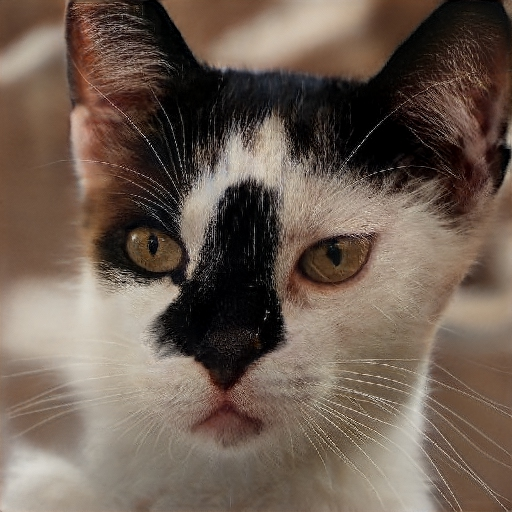
\includegraphics[width=0.2\textwidth]{dogs_cats/cat1.jpeg}};
      \node[anchor=south west,inner sep=0] (cat2) at (0,3) {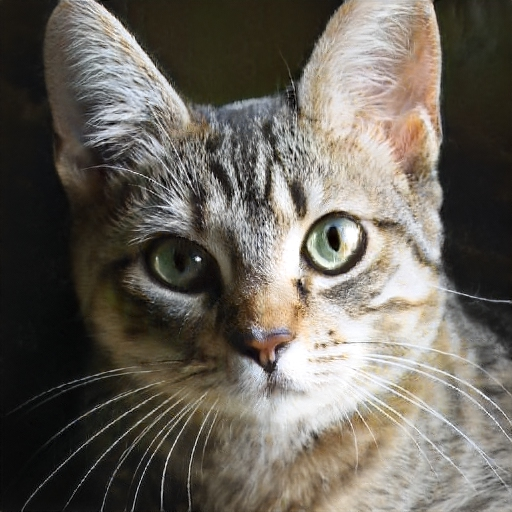
\includegraphics[width=0.2\textwidth]{dogs_cats/cat2.jpeg}};
      \node[anchor=south west,inner sep=0] (cat3) at (0,1.5) {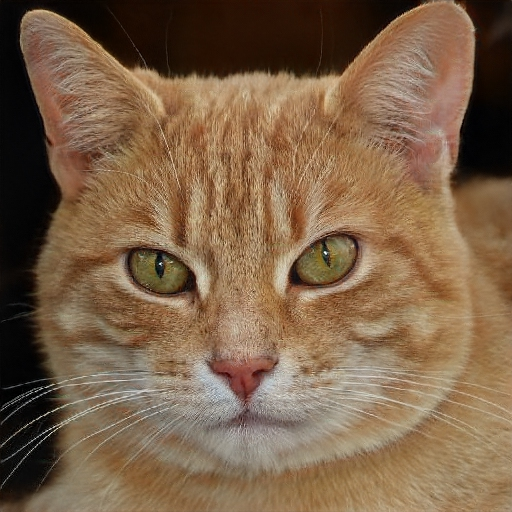
\includegraphics[width=0.2\textwidth]{dogs_cats/cat3.jpeg}};
      \node[anchor=south west,inner sep=0] (dog1) at (0,0) {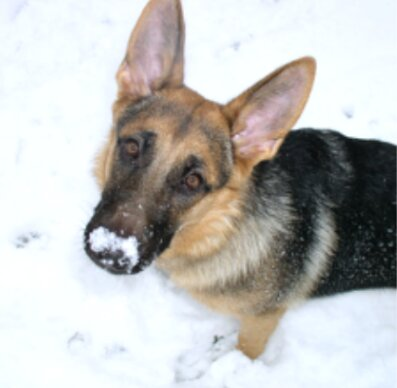
\includegraphics[width=0.2\textwidth]{dogs_cats/dog1.jpeg}};
      \node[anchor=south west,inner sep=0] (name1) at (2,4.75) {cat};
      \node[anchor=south west,inner sep=0] (name2) at (2,3.25) {cat};
      \node[anchor=south west,inner sep=0] (name3) at (2,1.75) {cat};
      \node[anchor=south west,inner sep=0] (name4) at (2,0.25) {dog};
      \draw [-latex,shorten >= 3pt, shorten <= 3pt, amaranth, ultra thick] (cat1) to (name1);
      \draw [-latex,shorten >= 3pt, shorten <= 3pt, amaranth, ultra thick] (cat2) to (name2);
      \draw [-latex,shorten >= 3pt, shorten <= 3pt, amaranth, ultra thick] (cat3) to (name3);
      \draw [-latex,shorten >= 3pt, shorten <= 3pt, amaranth, ultra thick] (dog1) to (name4);
  \end{tikzpicture}%
  \end{minipage}%
  \begin{minipage}{.5\textwidth}
    Goal:

    \vspace{0.5em}

    \Large
    \hspace{1em}
    learn
    a model $h_w$

    \hspace{1em}
    of the relation
    \begin{tikzpicture}
      \node (test) at (0, 0) {};
      \draw [-latex,shorten >= 3pt, shorten <= 3pt, amaranth, ultra thick] (0,0) to (1.5, 0);
    \end{tikzpicture}%
  \end{minipage}
  \end{center}

\end{frame}



\begin{frame}
    \vspace{1em}
  {\Huge
    \begin{center}
      Empirical Risk Minimization
    \end{center}
  }
  \vspace{-0.5em}
  \begin{align*}
    \argmin_{w \in \RR^p} f(w) = \frac 1n \sum_{i=1}^n \ell(h_w(x_i); y_i)
  \end{align*}

  \vspace{1.5em}

  {\Large
  Assumptions:
  \begin{itemize}
  \item $w \mapsto \ell(h_w(x_i),y_i)$ is convex, Lipschitz, and
    smooth
  \end{itemize}
  }

\end{frame}

\begin{frame}
  \begin{center}
    \vspace{2em}
    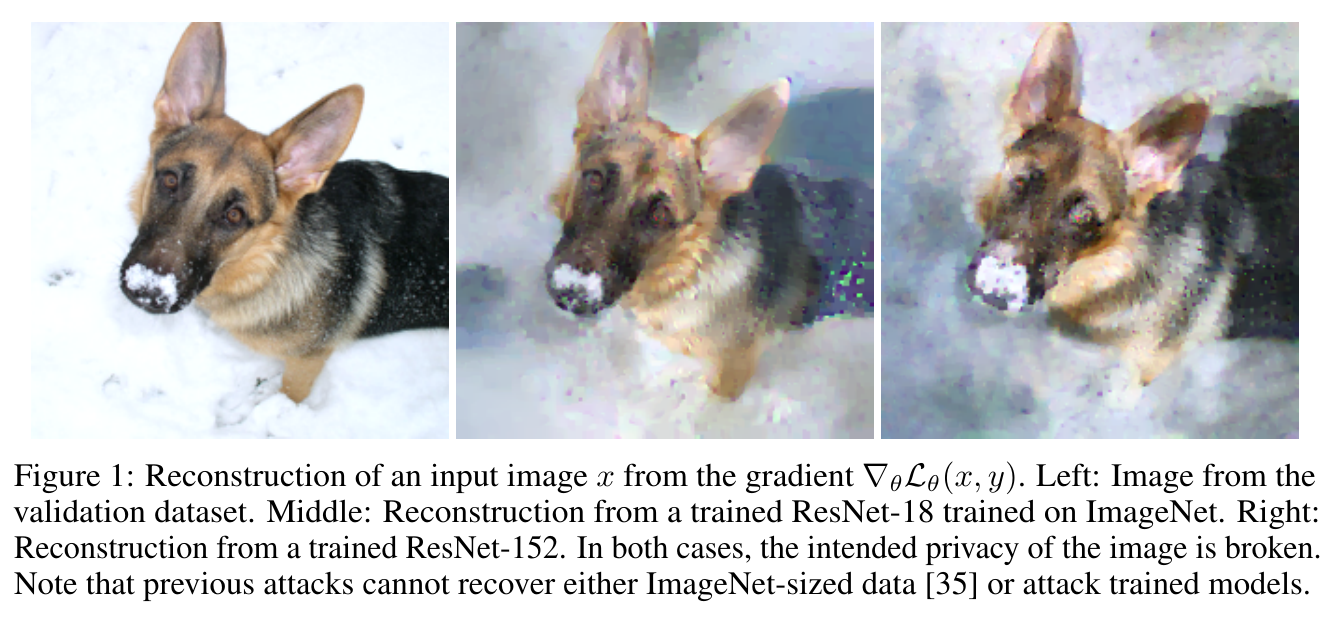
\includegraphics[width=1\linewidth]{reconstruction_attack.png}
  \end{center}

  \vspace{-1em}
  \smalllongcite{geiping2020Inverting}
\end{frame}

\begin{frame}
  \vspace{2em}

  {\Huge
    \begin{center}
      Differentially private ERM
    \end{center}
  }
  \vspace{-1.5em}
  \begin{align*}
    & \argmin_{w \in \RR^p} f(w) = \frac 1n \sum_{i=1}^n \ell(h_w(x_i); y_i) \\
    & \qquad \text{such that $w$ is $(\epsilon, \delta)$-DP}
  \end{align*}

  \vspace{-1em}

  \smalllongcite{chaudhuri2011Differentially}
\end{frame}

\begin{frame}
  \vspace{2em}

  $\emphcolb{\cA} : D \mapsto w$ is
  $(\emphcol{\epsilon}, \emphcol{\delta})$-\emph{Differentially
    Private}
  \begin{align*}
    \prob{\emphcolb{\cA}(D) \in \cS} \le e^{\emphcol{\epsilon}} \prob{\emphcolb{\cA}(D') \in \cS} + \emphcol{\delta}.
  \end{align*}

  \vspace{1em}

  \begin{flushright}
    ($D$ and $D'$ differ on one element.)
  \end{flushright}

  \smalllongcite{dwork2006Differential}
\end{frame}


\begin{frame}
  \vspace{0.5em}
  \begin{center}
    {\huge ``Distributions are similar''}

  \pause

  \vspace{1.5em}

    \begin{tikzpicture}
      \node [anchor=west] (td1) at (1,5) {\Large {Trained on $D$}};
      \node [anchor=west] (td2) at (7,5) {\Large {Trained on $D'$}};
      \node [anchor=west] (models) at (7, -0.5) {\Large {Models}};
      \begin{scope}[xshift=1.5cm]
        \node[anchor=south west,inner sep=0] (image) at (0,0) {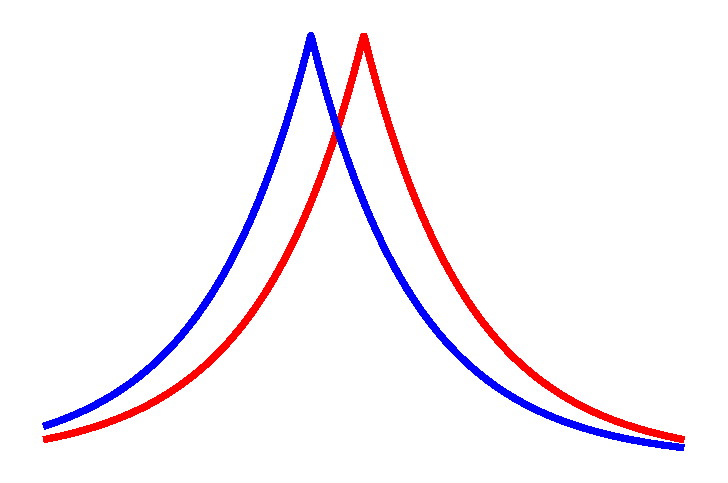
\includegraphics[width=0.7\textwidth]{distrib.pdf}};
        \begin{scope}[x={(image.south east)},y={(image.north west)}]
%          \draw[red,ultra thick,rounded corners] (0.48,0.80) rectangle (0.55,0.95);
          \draw [-latex, ultra thick, blue] (td1) to[out=270, in=150] (0.3,0.70);
          \draw [-latex, ultra thick, red] (td2) to[out=270, in=30] (0.6,0.70);
          \draw [-latex] (-0.1, 0) to (1.1,0);
        \end{scope}
      \end{scope}
    \end{tikzpicture}%
  \end{center}
\end{frame}


\begin{frame}

  \vspace{1em}

  \Huge\centering
  Solving DP-ERM?

  % \resizebox{5cm}{!}{
  %   \begin{minipage}{1.0\linewidth}
  %     \begin{align*}
  %       & \argmin_{w \in \RR^p} F(w) = f(w) + \psi(w)\\
  %       & \qquad \text{such that $w$ is $(\epsilon, \delta)$-DP.}
  %     \end{align*}
  %   \end{minipage}
  % }

  % \vspace{1em}
  % \pause
  % \Large
  % The classical: DP-SGD. \pause \\
  % The challenger: DP-CD.
\end{frame}

\begin{frame}
  \only<2>{\addtocounter{framenumber}{1}}
  \vspace{2em}
  \begin{center}
  {\huge \only<2>{Private }Stochastic Gradient Descent}
  \vspace{1em}
  \begin{align*}
    w^{t+1} = w^t - \eta
    \only<1>{\emphcol{\xi}}
    \only<2>{\left( \emphcol{\xi} + \emphcolb{\cN(\sigma^2\bbI)} \right)},
  \end{align*}

  \vspace{1em}

  where $\expec{}{\emphcol{\xi}} = \nabla f(w^t)$.
  \end{center}
\end{frame}


\begin{frame}
  \vspace{1em}

  \begin{center}
    \Huge Utility?
  \end{center}

  \begin{align*}
    \expec{}{f(w^T)-f^*} \le ~?
  \end{align*}
\end{frame}

\begin{frame}
  \huge
  \vspace{1em}

  \begin{center}

  Convex loss: $O\left( \frac{\emphcol{\sqrt{p}}}{n\epsilon} \right)$

  Strongly-Convex loss: $O\left( \frac{\emphcol{p}}{\mu n^2\epsilon^2} \right)$

  \vspace{2em} \pause

  \huge
  \emph{Polynomial dependence on $p$... \Frowny{}}

  \pause
  \vspace{0.5em}

  Can not be improved in general. \Frowny{}\Frowny{}
  \end{center}
\end{frame}


\begin{frame}
  \vspace{1em}
  \begin{center}
    \Huge Look at our gradient!
  \end{center}

  \vspace{-2.32em}

  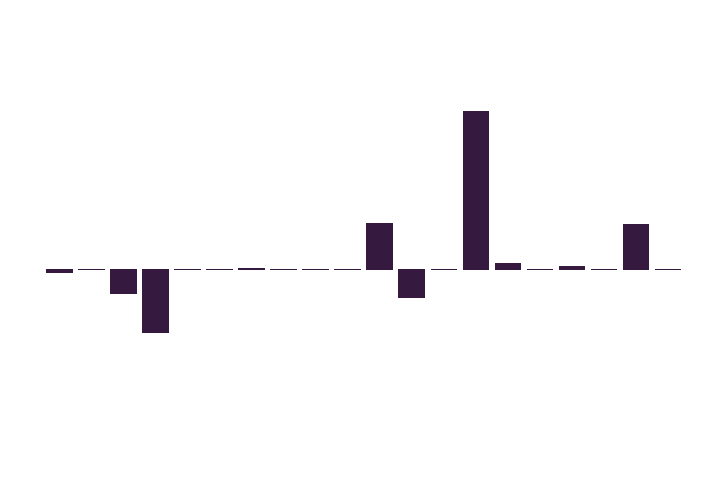
\includegraphics[width=\textwidth]{grad_example_1.pdf}

  \vspace{-2em}

  \begin{center}
    \phantom{\Huge Noise scales with dimension. \Frowny{}}
  \end{center}
\end{frame}

\begin{frame}
  \vspace{1em}

  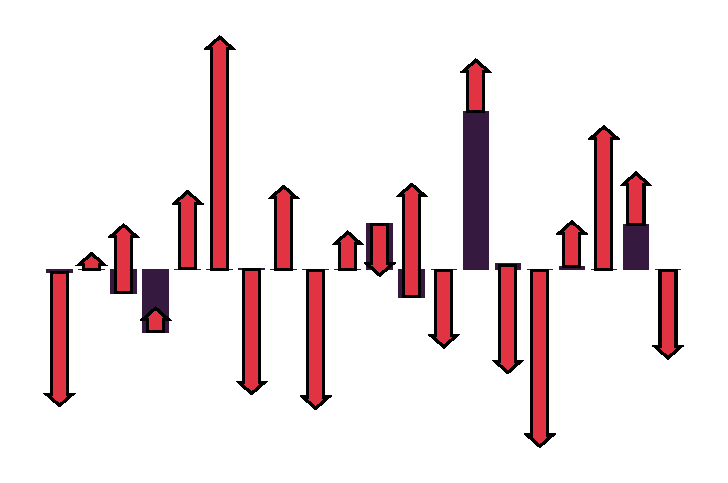
\includegraphics[width=\textwidth]{grad_example_2.pdf}

  \vspace{-1.5em}

  \begin{center}
    \Huge Noise scales with dimension. \Frowny{}
  \end{center}
  \addtocounter{framenumber}{-1}
\end{frame}

\begin{frame}
  \vspace{1em}

  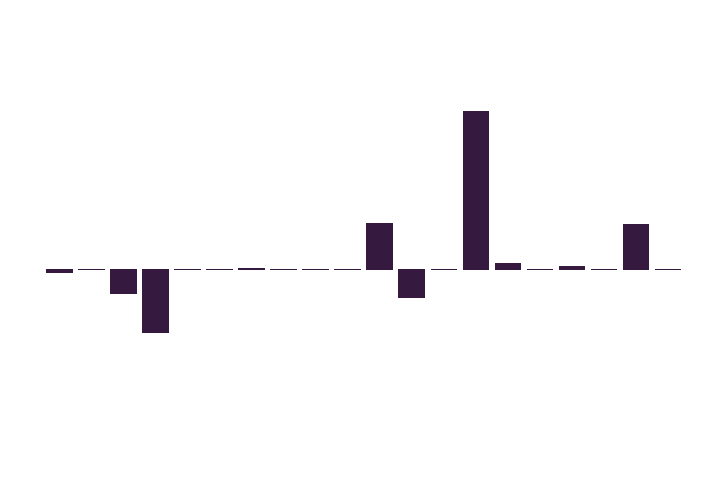
\includegraphics[width=\textwidth]{grad_example_1.pdf}

  \vspace{-2em}

  \begin{center}
    {\Huge Release only the maximum?}
  \end{center}
\end{frame}


\begin{frame}
  \vspace{1em}

  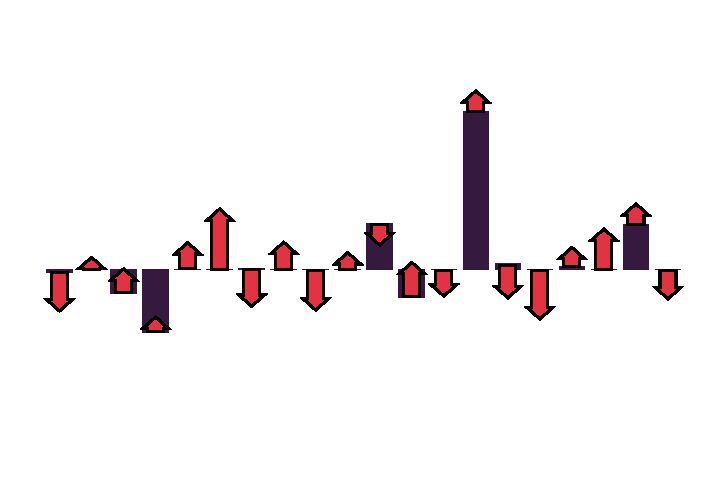
\includegraphics[width=\textwidth]{grad_example_noisy_1.pdf}

  \vspace{-1.5em}

  \begin{center}
    \Huge Noise is \emph{much} smaller! \Smiley{}
  \end{center}
  \addtocounter{framenumber}{-1}
\end{frame}

\begin{frame}
  \vspace{1em}

  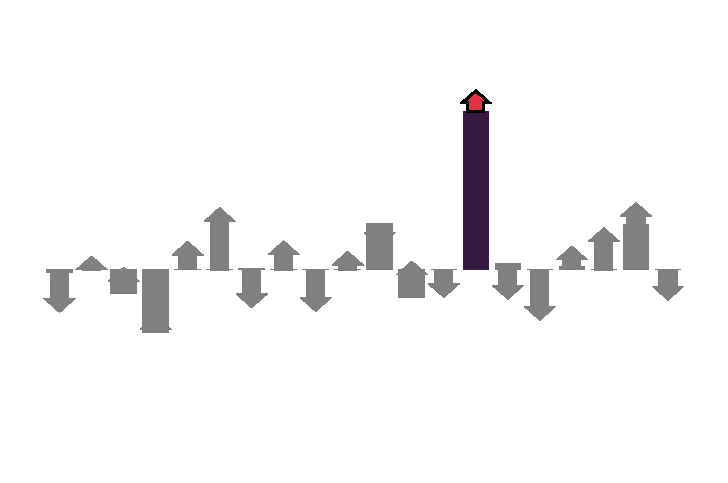
\includegraphics[width=\textwidth]{grad_example_3.pdf}

  \vspace{-3em}

  \begin{center}
    \Huge But: we can use only \textsc{ONE} coordinate.
  \end{center}
  \addtocounter{framenumber}{-1}
\end{frame}



\begin{frame}
  \vspace{2em}

  \begin{center}
    {\huge Private \emph{Greedy} Coordinate Descent}
  \end{center}
  \begin{align*}
    & \text{Choose} \\
    & \quad j = \argmax_{j'\in[p]} \abs{\emphcol{\nabla_{j'} f(w^t)} + \emphcolb{\Lap(\lambda_{j'}')}} \\
    & \text{Update} \\
    & \quad w^{t+1}_{j} =
      w^t_{j} - \eta_{j}
    \left( \emphcol{\nabla_{j} f(w^t)}
    + \emphcolb{\Lap(\lambda_{j})} \right)
  \end{align*}
\end{frame}


\begin{frame}
  \huge
  \vspace{1em}

  \begin{center}

    Under favorable structure, we obtain:

    \vspace{1.5em}

    Convex loss: $O\left( \frac{\emphcol{\log{p}}}{n\epsilon} \right)$

    Strongly-Convex loss: $O\left( \frac{\emphcol{\log{p}}}{\mu^2 n^2\epsilon^2} \right)$

  \vspace{2em} \pause

  \huge
  \emph{Logarithmic dependence on $p$!!! \Smiley{}}

  \vspace{0.5em}

  \end{center}
\end{frame}

\hspace{-3.3em}
\begin{frame}
  \vspace{-0.3em}
  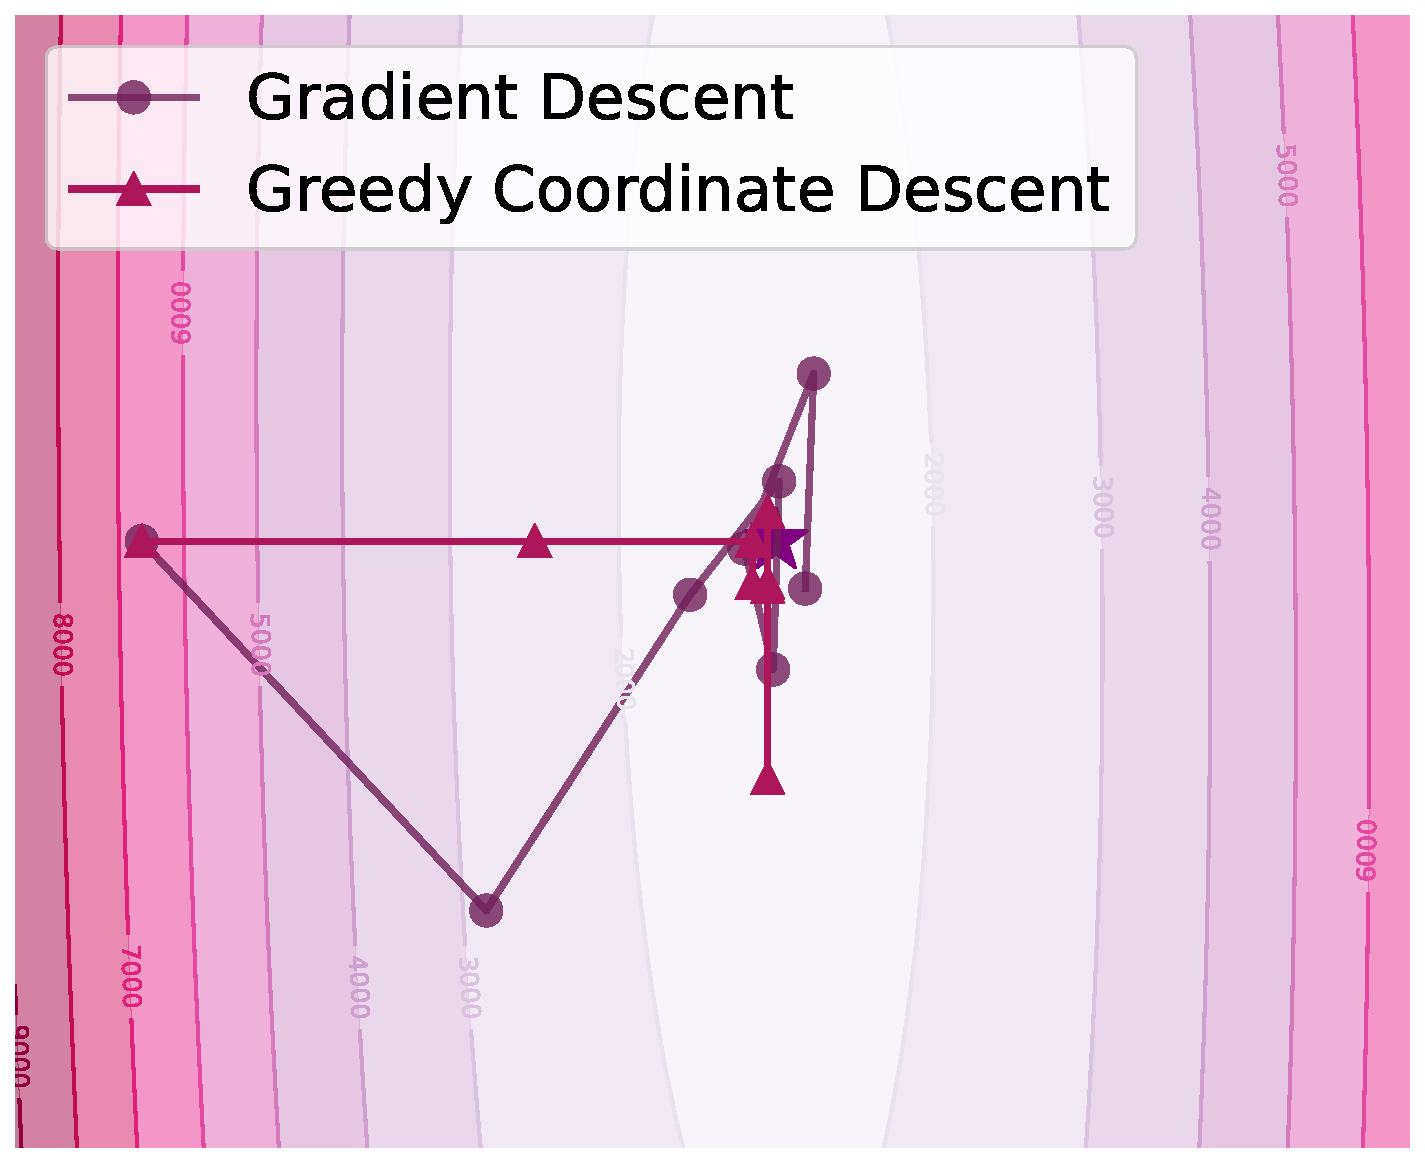
\includegraphics[width=1.17\textwidth]{example_3.pdf}
\end{frame}

\begin{frame}

  \begin{center}
    {\huge Wrap-up!}

    \vspace{1em}

    \begin{itemize}
    \item Models contain sensitive information.
    \item Training can be done privately.
    \item Greedy approaches can help.
    \end{itemize}
  \end{center}
\end{frame}

\end{document}
%%% Local Variables:
%%% mode: latex
%%% TeX-master: t
%%% End:
